\begin{figure}[htbp]
\centering
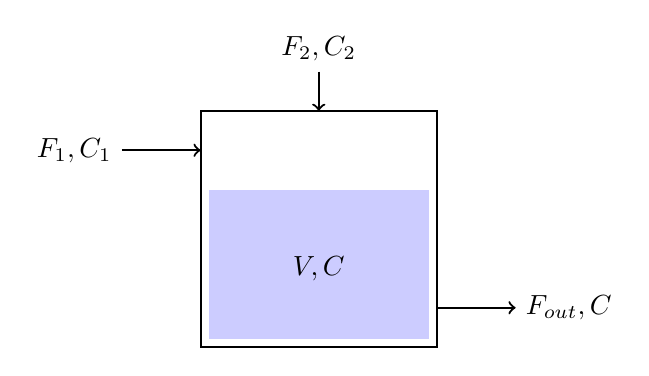
\begin{tikzpicture}
    % Tank
    \draw[thick] (0,0) -- (0,3) -- (3,3) -- (3,0) -- cycle;
    \fill[blue!20] (0.1,0.1) rectangle (2.9,2);

    % Inlet 1
    \draw[->, thick] (-1,2.5) -- (0,2.5) node[left, pos=0] {$F_1, C_1$};

    % Inlet 2
    \draw[->, thick] (1.5,3.5) -- (1.5,3) node[above, pos=0] {$F_2, C_2$};

    % Outlet
    \draw[->, thick] (3,0.5) -- (4,0.5) node[right] {$F_{\text{out}}, C$};

    % Labels
    \node at (1.5,1) {$V, C$};
\end{tikzpicture}
\caption{Mixing tank with two inlets.}
\label{fig:mixing_tank}
\end{figure}
